\chapter{Grundlegendes}
\label{cha:grundlegendes}
% 3 Seiten

\section{Definition}

Deep Learning ist ein Ansatz aus dem maschinellen Lernen, der sich mit dem Trainieren von nichtlinearen Modellen und hier meist mit vielschichtigen neuronalen Netzen befasst. 

Deep Learning wird zum Beispiel zur Klassifizierung von Daten oder zur Extraktion von Merkmalen aus Daten eingesetzt.

\section{Entstehung}
\label{cha:entstehung}

Die Wurzeln neuronale Netze gehen zurück in die 1950er Jahre, als Frank Rosenblatt eine Maschine namens Perceptron \citep{Perceptron} beschrieb. Diese Maschine war in der Lage einige einfache Figuren wie Quadrate und Dreiecke zu erkennen. Für die damalige Zeit war das eine herausragende Maschine und regte den Gedanken, Maschinen zu bauen die Menschen imitieren können, weiter an.

Knapp 20 Jahre später schrieb Marvin Minsky \citep{PerceptronsMinsky} ein Buch das die Limitierungen von Preceptrons aufzeigte und einige scheinbar fundamentale Probleme aufwarf. Diese Erscheinung ließ die neuronalen Netze wieder in den Hintergrund rücken.
In den 1980er Jahren, hat der heute renommierte Wissenschaftler Geoff Hinton, neuronale Netze beschrieben \citep{BackpropagationEarly}, die bereits eine versteckte Schicht enthielten und somit in der Lage waren, komplexere Aufgaben zu lösen. In dieser Zeit entstand auch der Backpropagation Algorithmus für das Trainieren von neuronalen Netzen. %\todo{ref Werbos, Amari?, Parker, LeCun, Rumelhart, ..)}
Das trainieren dieser neuronalen Netze war sehr aufwendig und so verschwand auch sie bald wieder von der Bildfläche. 

Erst mit einer Entdeckung 2006 \citep{BackpropagationFast}, erneut durch Geoff Hinton, die den Backpropagation-Algorithmus erheblich vereinfachte, haben neuronale Netze mit mehreren versteckten Schichten wieder an Bedeutung gewonnen. 

Heute stellen führende Unternehmen immer häufiger Teams rund um die Thematik der neuronale Netze zusammen um sich wirtschaftliche Vorteile zu sichern \footnote{2013/3 Google stellt Geoffrey Hinton ein},\footnote{2013/12 Facebook stellt NYU Professor Yann LeCun ein}. Erste Erfolge sieht man an Microsofts Spracherkennung Cortana, Siri von Apple, Google Now oder der Bildersuche von Google, die anhand von Bildern ähnliche Bildern findet.


\section{Hürden}

Die aus der Vergangenheit bekannten Probleme des Lernens neuronaler Netze mit vielen versteckten Schichten strecken sich zum größten Teil bis heute durch. Zusätzliche versteckte Schichten erlauben es Modellen oft sich auf nicht repräsentative Abhängigkeiten der Trainingsdaten anzupassen und so tendieren vielschichtige neuronale Netze beim Training häufig zur Überanpassung. Problemstellen beim Training sind häufig auch die Unteranpassung durch zu wenig Trainingsdaten, lokalen Minima in denen die Trainingsalgorithmen hängen bleiben und die notwendige Rechenleistung.

Grundsätzlich kann man für heute verwendete Algorithmen sagen, dass die Leistung von neuronalen Netzen sehr stark von der Menge der Trainingsdaten und weniger von dem Trainingsalgorithmus selbst abhängt. Nicht zuletzt hat die Verfügbarkeit von immensen Datenmengen von Unternehmen und aus dem Internet einen sehr positiven Einfluss auf die Entwicklungen und damit das Interesse von Deep Learning.

%hidden layer nicht trainiert werden konnten (rechenpower außer bei time-delay und convolutional nets) + hat nicht für netzwerke mit feedback funktioniert

\section{Neuronale Netze}

\begin{figure}
	\centering
	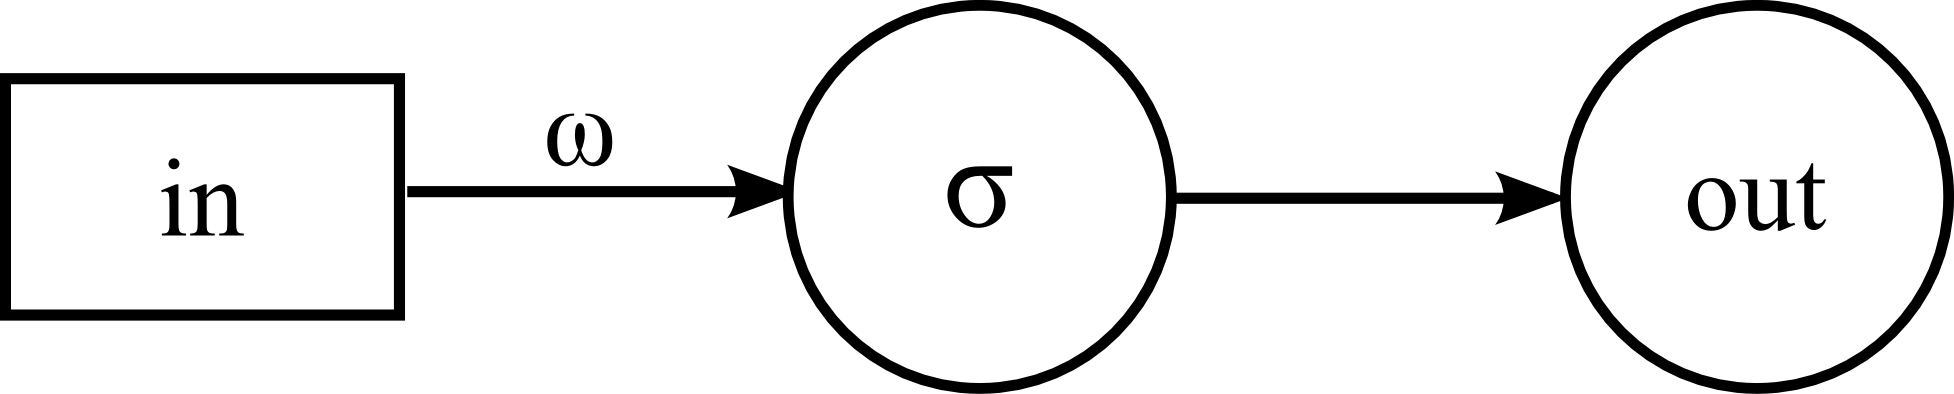
\includegraphics[scale=1]{images/neuron.png}
	\caption{Neuron}
	\label{fig:neuron}
\end{figure}

Künstliche neuronale Netze sind Strukturen aus der Technik, die dem Nervensystem von Lebewesen ähneln. Es sind Netze die aus Eingangsdaten Ausgangsdaten über nicht lineare Zusammenhänge berechnen. Diese Netze müssen parametrisiert werden. Hier kommt Deep Learning zum Einsatz.

Neuronale Netze sind in der Technik zur Vereinfachung meist in mehreren Schichten aufgebaut. Abbildung \ref{fig:neuron} zeigt ein einfaches Neuron mit nur einem Eingang. Der Ausgang wird aus der Multiplikation des Eingangswerts mit dem Gewicht und der Übertragungsfunktion $\sigma$ errechnet. Als Übertragungsfunktion wird meist die Sigmoid-Funktion eingesetzt, sie lässt sich einfach differenzieren \citep{sigmoid} und eignet sich daher besonders gut. Der Ausgang $out$ dieses Neurons ergibt sich somit aus der dem Eingang $in$ multipliziert mit dem Gewicht $\omega$ in der Sigmoid-Funktion $\sigma$.
$$out = \sigma(\omega * in)$$

\begin{figure}
	\centering
	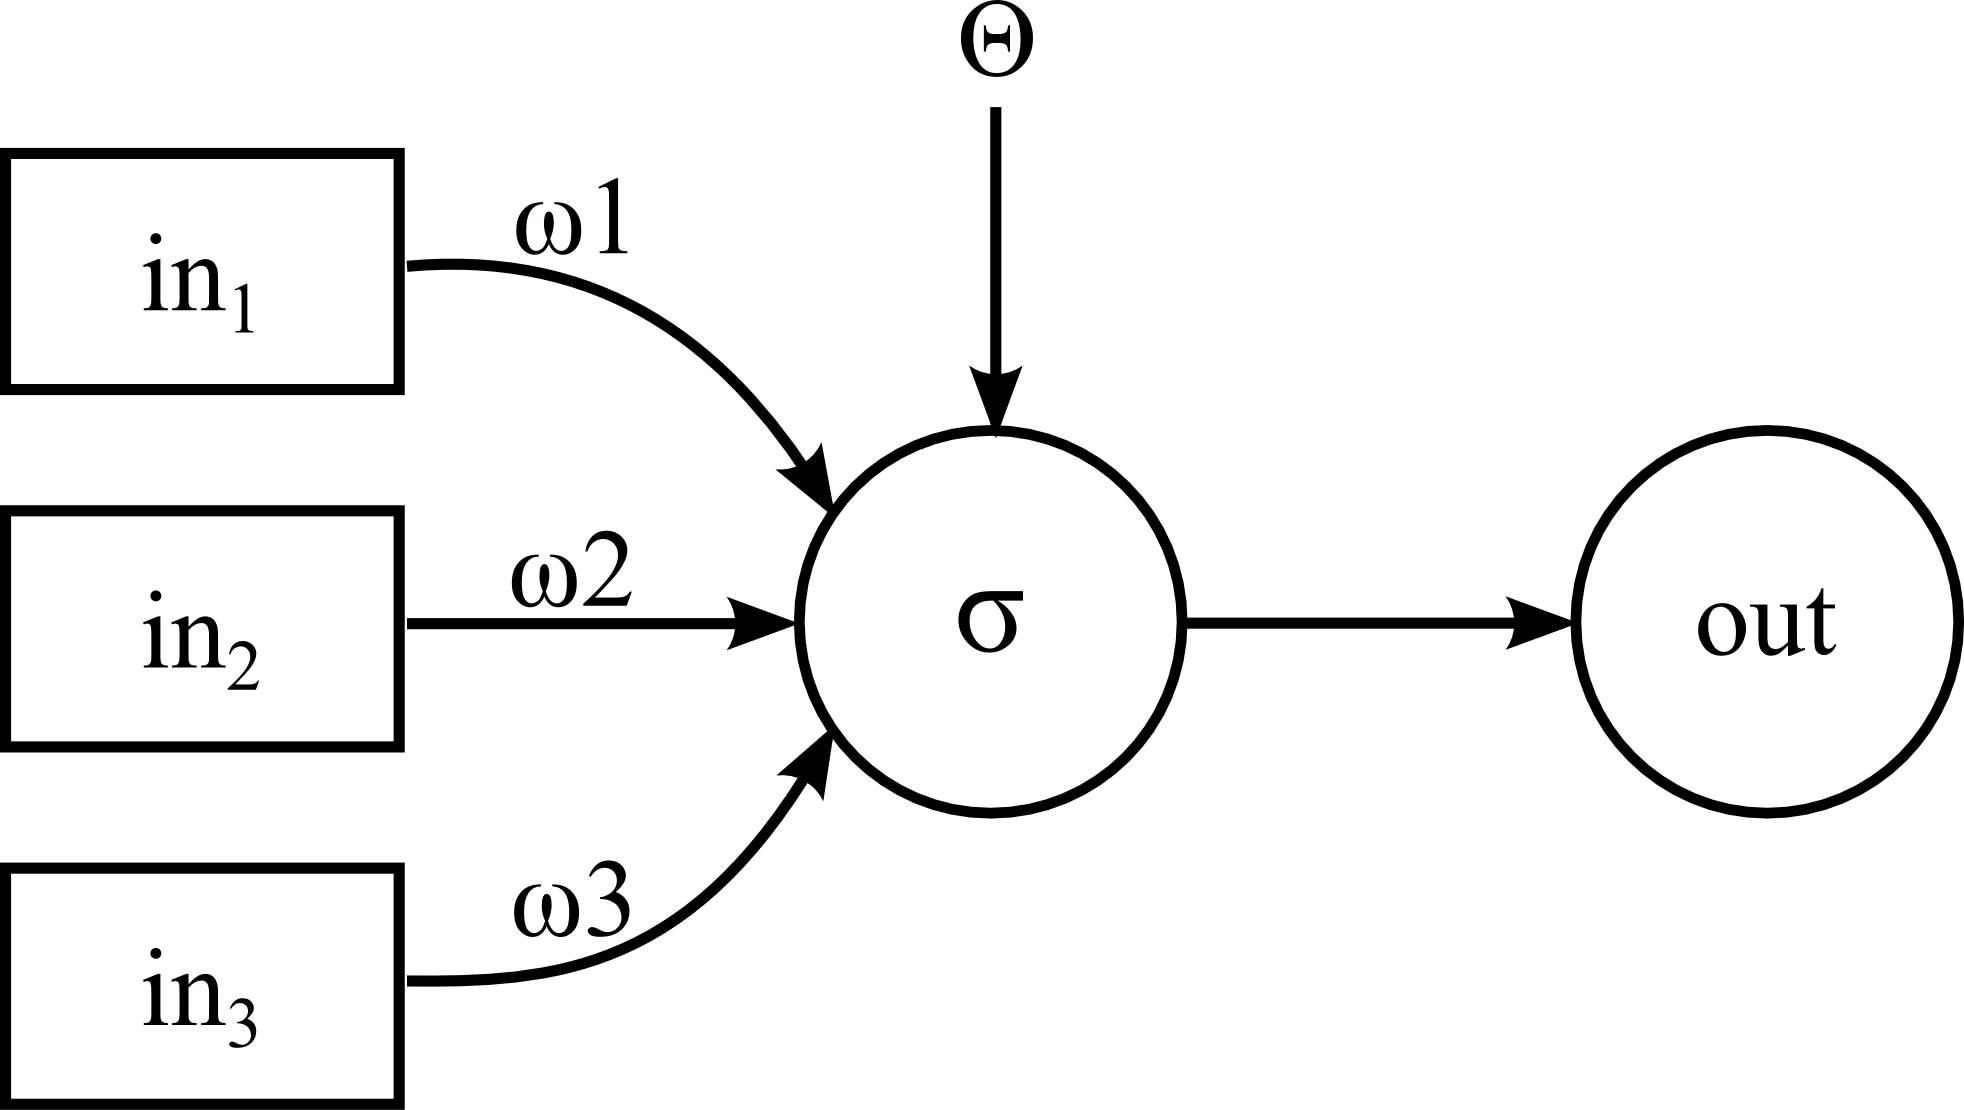
\includegraphics[scale=1]{images/neuron-multiple-inputs.png}
	\caption{Neuron mit mehreren Eingängen}
	\label{fig:neuron-multiple-inputs}
\end{figure}

Ein Neuron hat in der Regel, wie in Abbildung \ref{fig:neuron-multiple-inputs} zu sehen, mehrere Eingänge. Außerdem wird ein Bias-Wert $\theta$ für die Sigmoid-Funktion hinzugefügt. Der Ausgang dieses Neurons kann somit wie folgt berechnet werden:
$$out = \sigma(\omega_1*in_1 + \omega_2*in_2 + \omega_3*in_3 + \theta)$$

%\begin{figure}
%	\centering
%		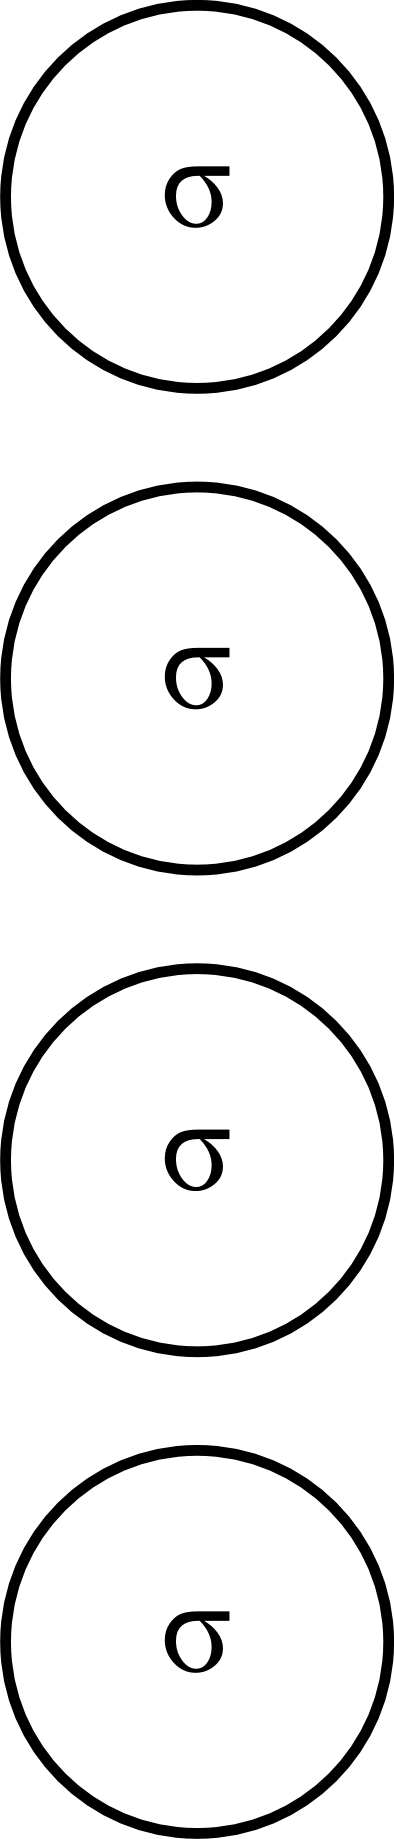
\includegraphics[scale=1]{images/neuron-layer.png}
%	\caption{Schichten von Neuronen}
%	\label{fig:neuron-layer}
%\end{figure}

\begin{figure}
	\centering
		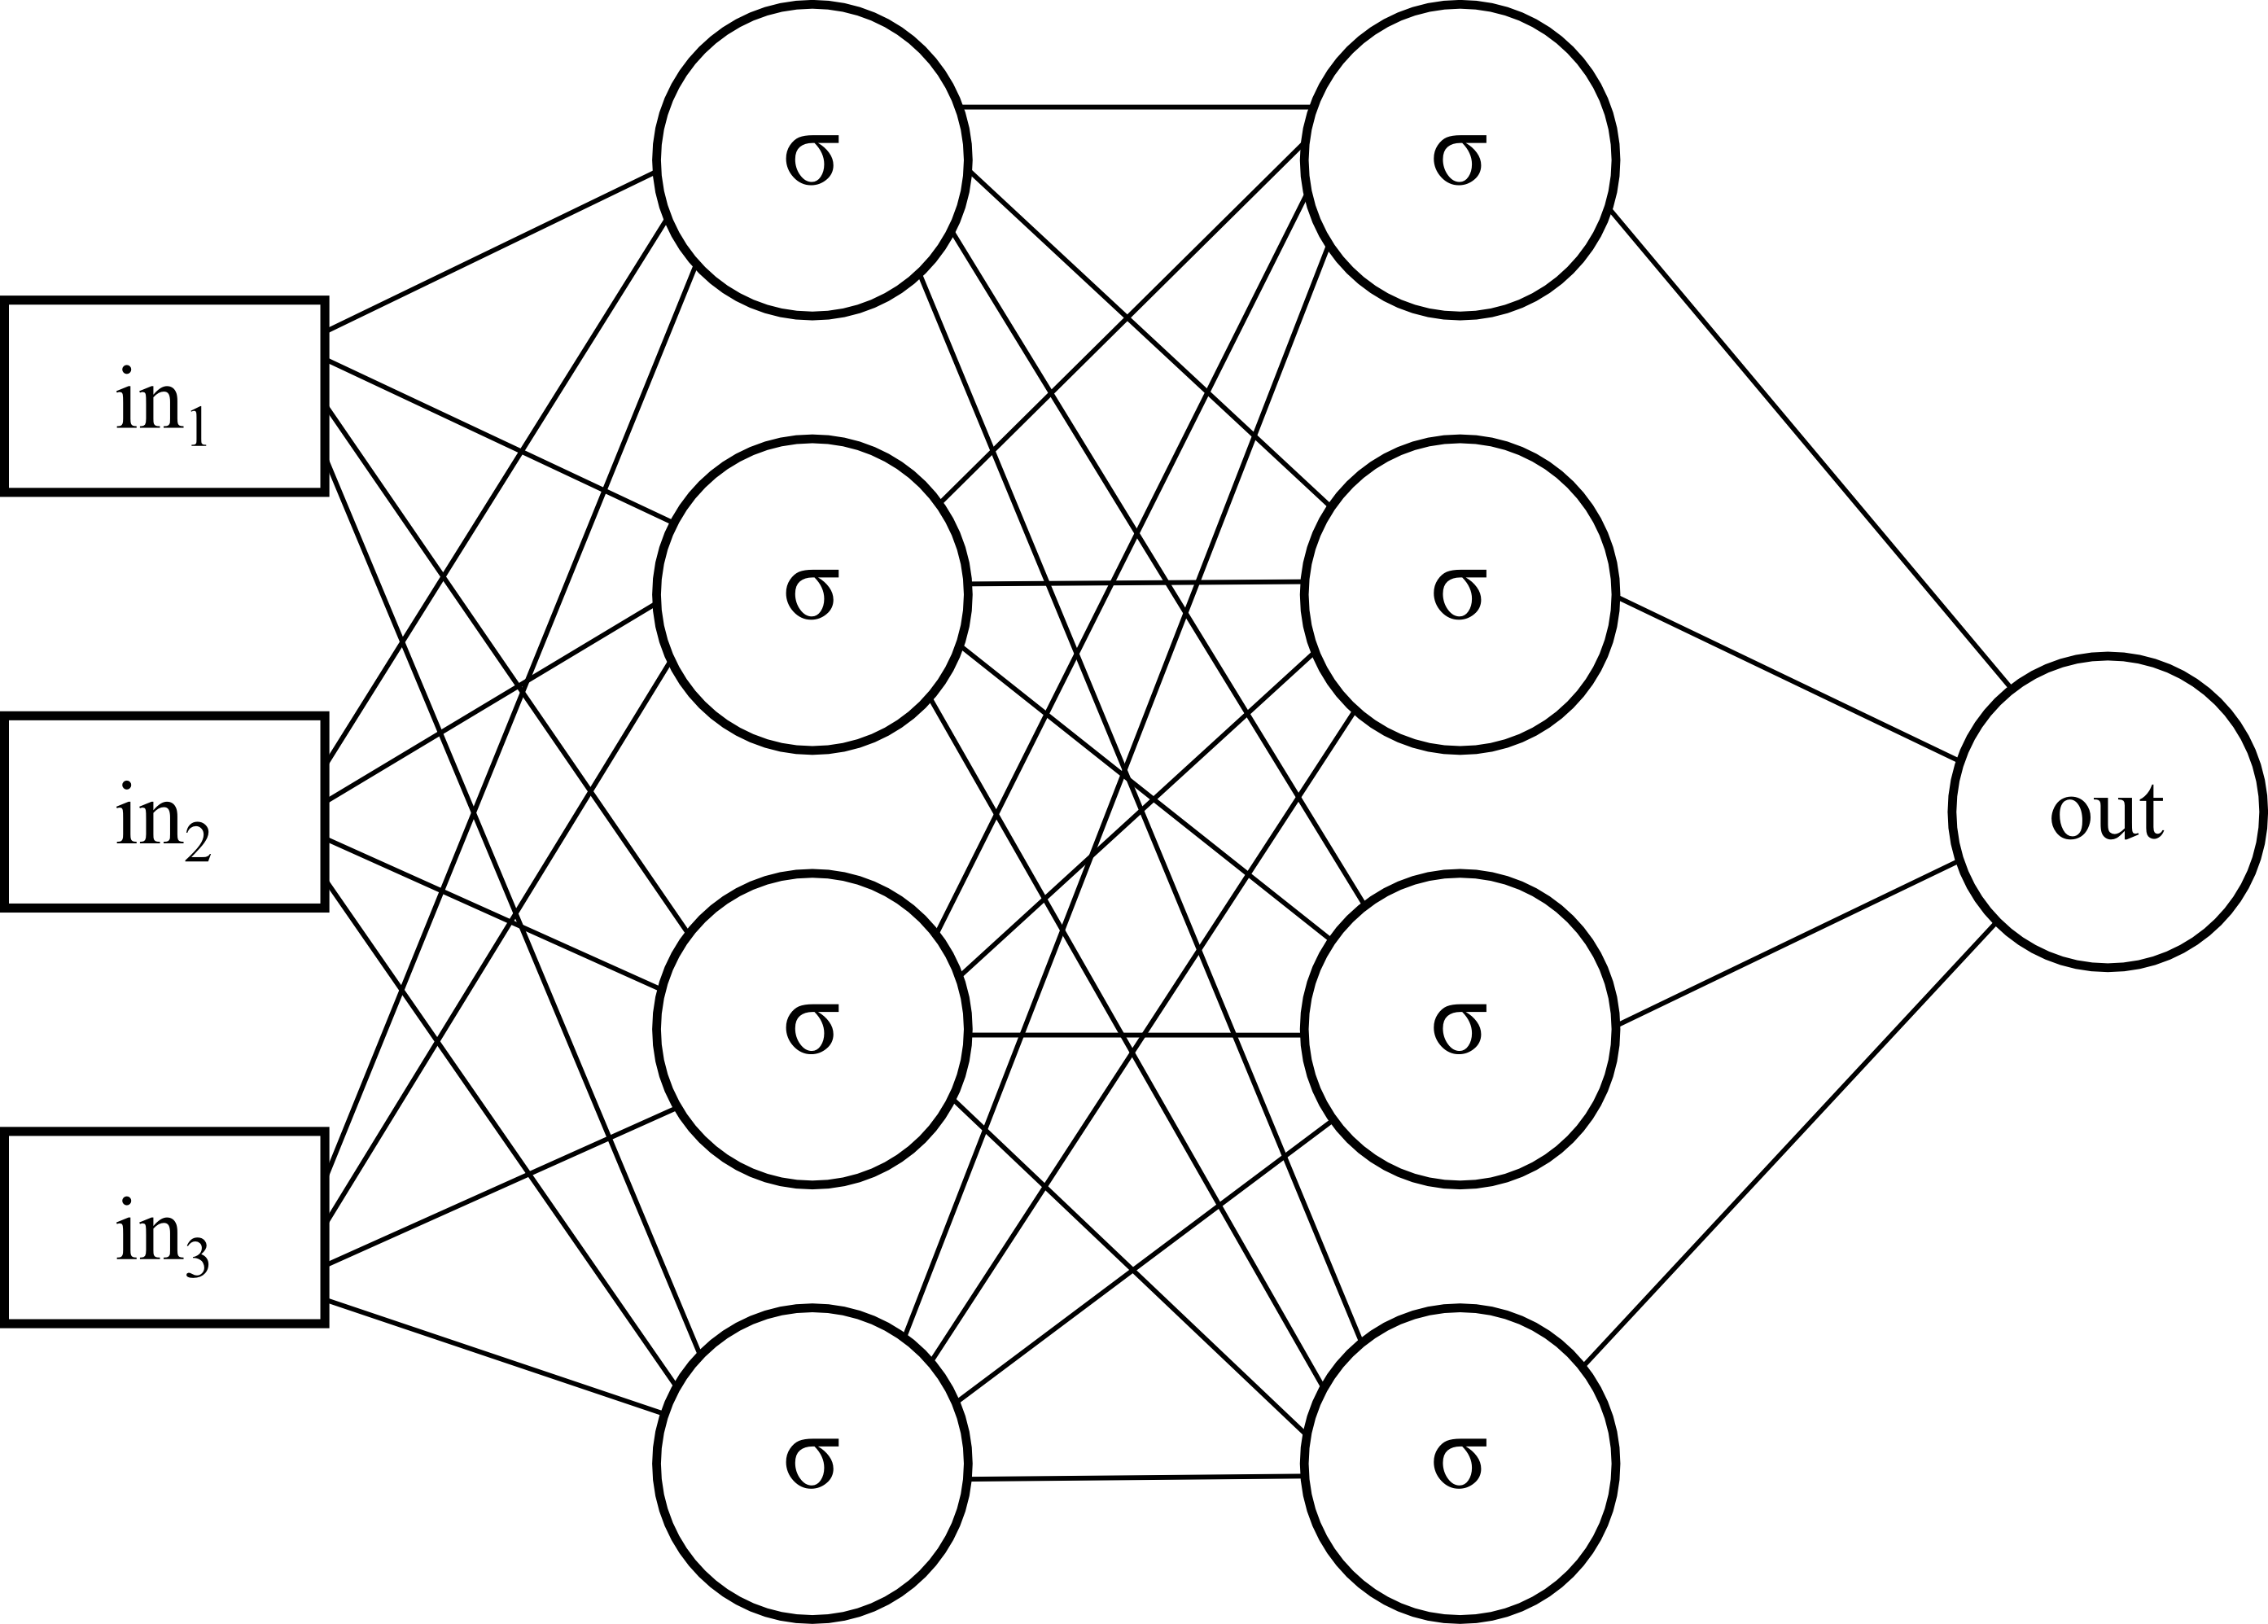
\includegraphics[scale=1]{images/neuron-network.png}
	\caption{Ein neuronales Netz}
	\label{fig:neuron-network}
\end{figure}

Um aus den einzelnen Neuronen ein Netzwerk zu bauen, werden Schichten gebildet. Eine Schicht ist eine Menge an Neuronen, die, zur Vereinfachung, untereinander meist nicht direkt verknüpft sind. Schichten werden hintereinander gehängt, in dem jedes Neuron einer Schicht als Eingang für jedes Neuron der nächsten Schicht dient. Ein solches Netzwerk ist auch in Abbildung \ref{fig:neuron-network} zu sehen. Dieses Netzwerk hat eine Eingabeschicht, eine Ausgabeschicht und zwei Schichten dazwischen. Da die Ergebnisse dieser mittleren Schichten in der Regel nicht unmittelbar ein Ergebnis sind, werden sie als unsichtbar betrachtet und auch so bezeichnet. Es handelt sich hierbei also um die versteckten Schichten.

\section{Überwachtes / unüberwachtes Lernen}

Die Algorithmen des Deep Learnings werden im groben in zwei Kategorien geteilt, in die überwachten und die unüberwachten Methoden. Überwacht bedeutet, dass Eingangsdaten an das System angelegt werden für die die gewünschten Ausgangsdaten bekannt sind. Das könnte zum Beispiel heißen, dass das Netz mit Bilder trainiert wird, von denen einige Gesichter enthalten und einige nicht. Am Ausgang wird dann überprüft ob das Netz die Gesichter richtig erkannt hat und wenn nicht, werden die Parameter des Netzes entsprechend angepasst.

Diese Art des Lernens scheint logisch, benötigt aber sehr viele Datensätze mit bekannten Ausprägungen. Deklarierte Datensätze sind selten in großen Mengen verfügbar und so tendiert diese Art der Algorithmen leicht zur Überanpassung \citep{overfitting}, mehr dazu bei den jeweiligen Algorithmen.

Ein weitere Ansatz ist das unüberwachte Lernen, es handelt sich dabei um Algorithmen, die Eingangsdaten aber keine Ausgabedaten zum Vergleich benötigen. Die grundlegende Idee dabei ist es, das Netz Merkmale aus den Eingangsdaten lernen zu lassen. Unüberwachtes Lernen ist besonders wegen der großen Verfügbarkeit unkategorisierten Daten interessant und wird häufig als Grundlage vor dem überwachten Lernen eingesetzt. Es hilft einige Probleme des überwachten Lernens zu verbessern, so können die Gewichte aus dem unüberwachten Lernen als Startwert für ein überwachtes Lernen eingesetzt werden \citep{preunsupervised}. Diese Gewichte haben mehr Aussagekraft über Merkmale der Eingangsdaten als zufällige Werte und können mit weniger kategorisierten Trainingsdaten oft wesentlich bessere Ergebnisse erzielt werden.